\documentclass[12pt,a4paper]{article}
\usepackage{fullpage}
\usepackage[margin=2cm]{geometry}
\usepackage{amsmath}
\usepackage{subfig}
\usepackage{graphicx}
\usepackage[justification=centering]{caption}
\begin{document}
\title{Fine-tuning ImageNet on Beetles datasets}
\author{LE Van Linh}
\date{\today}
\maketitle
\begin{abstract}
	In this study, we fine-tune on some trained models on pronotum dataset, such as VGG, GoogleNet, ResNet50. In some case, we use the model which have been designed for classification problem to adapt to a regression problem. The experiments will implement on two steps: freeze and unfreeze some layers in trained models. At the end of the experiment, a comparison between the fine-tune losses will be discussed.
\end{abstract}
\section{Dataset}
The dataset includes 293 RGB-images of beetle's pronotum. The images were taken by the same camera with the same conditions of resolution of $3264 \times 2448$. The images in the dataset were divided into two subsets: training (including $260$ images) and testing (including $33$ images). For each image, a set of 8 manual landmarks have been set by biologists. Depending the input of the pre-trained models, the images are down-sampled to fit with the models. Firstly, the images are down-sampled to a resolution of $326 \times 245$ and the coordinates of the manual landmarks are also re-scaled. Secondly, the centroid point of manual landmarks is calculated for each image. The centroid point is considered as the center of the new image that has been cropped from the down-sampled image. The size of the new image is depending on the input of the trained model that we would like to fine tune. Fig. \ref{figdata} presents an example in dataset after down-sampling and crop the image to fit with the input size of neural network.

\begin{figure}[h!]
\centering
\subfloat[]{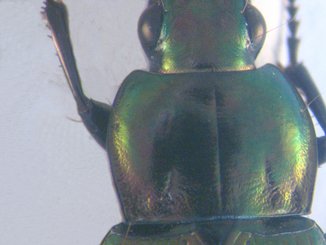
\includegraphics[scale=1.1]{./images/imagenet_finetuning/Prono_001_326}\label{a1}}\hspace{1cm}
\subfloat[]{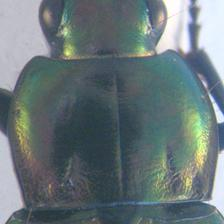
\includegraphics[scale=0.5]{./images/imagenet_finetuning/Prono_001_224}{\label{a2}}}
\caption{An example in dataset. \textit{a)} presents the image after down-sampling. \textit{b)} presents the cropped image from down-sampling image which used as the input of CNN}
\label{figdata}
\end{figure}
\section{The models}
\subsection{VGGs models}
The models are the improved versions of the models used by the VGG team in ILSVRC-2014 competition. The models were designed to evaluate the depth of the network by using an architecture with very small ($3 \times 3$) convolution filters and pushing the depth to $16 \to 19$ weight layers. Table. shows the architecture of the VGGs models.

\begin{table}[h!]
	\centering
	\begin{tabular}{c l l}
	Layer & $VGG-16$ & $VGG-19$ \\ \hline
	0 & Input(3,224,224) & Input(3,224,224) \\ \hline
	1 & CONV(64,3,1) & CONV(64,3,1) \\ \hline
	2 & CONV(64,3,1) & CONV(64,3,1) \\ \hline
	3 & POOL(2) &  POOL(2) \\ \hline
	4 & CONV(128,3,1) & CONV(128,3,1) \\ \hline
	5 & CONV(128,3,1) & CONV(128,3,1) \\ \hline
	6 & POOL(2) &  POOL(2) \\ \hline
	7 & CONV(256,3,1) & CONV(256,3,1) \\ \hline
	8 & CONV(256,3,1) & CONV(256,3,1) \\ \hline
	9 & CONV(256,3,1) & CONV(256,3,1) \\ \hline
	10 & POOL(2) &  CONV(256,3,1) \\ \hline
	11 & CONV(512,3,1) & POOL(2) \\ \hline
	12 & CONV(512,3,1) & CONV(512,3,1) \\ \hline
	13 & CONV(512,3,1) & CONV(512,3,1) \\ \hline
	14 & POOL(2) &  CONV(512,3,1) \\ \hline
	15 & CONV(512,3,1) & CONV(512,3,1) \\ \hline
	16 & CONV(512,3,1) & POOL(2) \\ \hline
	17 & CONV(512,3,1) & CONV(512,3,1) \\ \hline
	18 & POOL(2) &  CONV(512,3,1) \\ \hline
	19 & FC(4096) & CONV(512,3,1) \\ \hline
	20 & DROP(0.5) & CONV(512,3,1) \\ \hline
	21 & FC(4096) & POOL(2) \\ \hline
	22 & DROPOUT(0.5) &  FC(4096) \\ \hline
	23 & FC(1000) & DROP(0.5) \\ \hline
	24 & - & FC(4096) \\ \hline
	25 & - &  DROP(0.5) \\ \hline
	26 & - &  FC(1000) \\ \hline
	\end{tabular}
	\caption{The architecture of VGG-16 and VGG-19}
	\label{VGGmodels}
\end{table}

The parameters of CNN are shown in Table.x.
\begin{table}[h!]
	\centering
	\begin{tabular}{l l l}
	Parameter & Initial value & End value \\ \hline
	Epochs & 10000 &  \\ \hline
	Training batch size & 128 & \\ \hline
	Testing batch size & 128 & \\ \hline
	Learning rate & 0.03 & 0.0001 \\ \hline
	Momentum & 0.9 & 0.9999 \\ \hline
	\end{tabular}
	\caption{The network parameters in proposed model}
	\label{model2parameters}
\end{table}
\subsection{ResNet model}
\section{Experiments}
The dataset includes 260 image in 3-channels was used to fine-tune on each trained model. Table.\ref{result} shows the losses during fine-tuning (training and validation loss). During fine-tuning, the learning rate and momentum were kept the same on all trained model ($0.000001$ and $0.9$, respective). Each model was fine-tuned in two steps: \textit{freeze and un-freeze} some ``lower" layers in $5000$ epochs.

\begin{table}[h!]
	\centering
	\begin{tabular}{l l l}
	Model & Training loss & Validation loss \\ \hline
	VGG-16 (unfreeze) & 11.00030 & 9.41890  \\ \hline
	VGG-16 (freeze) & 0 & 0 \\ \hline
	VGG-19 (unfreeze) & 0 & 0 \\ \hline
	VGG-19 (freeze) & 0 & 0 \\ \hline
	ResNet (unfreeze) & 0 & 0 \\ \hline
	ResNet (freeze) & 0 & 0 \\ \hline
	\end{tabular}
	\caption{The losses during fine-tuning the trained models}
	\label{result}
\end{table}

\section{Conclusions}
A CNN model has been trained on a dataset that includes the images of three parts of beetle. The trained model then has been fine-tuned with the pronotum dataset. Comparing the losses when we trained the pronotum from scratch, the losses during fine-tuning has been improved $40\%$ on validation test. Besides, the coordinates of predicted landmarks are also more accuracy than the last result (training from scratch) (Table.\ref{tab2}). From the result, we can see that fine-tuning has affected to the results from CNN. However, the effects still limits in our case. The experiments of the techniques on fine-tuning need to do to reach to the result as we expect.
\bibliographystyle{unsrt}
\bibliography{includes/references}

\end{document}